\documentclass[11pt]{article}
\usepackage{fullpage,times,epsfig,graphicx}
\usepackage{amsthm}
\usepackage{latexsym}
\usepackage{tabularx,multirow}
\usepackage[T1]{fontenc}
\usepackage[scaled=0.8]{luximono}
\usepackage{listings}
\usepackage{graphicx}
\usepackage{color}
\definecolor{light-grey}{RGB}{240,240,240}
\definecolor{grey}{RGB}{230,230,230}
\lstset{
	language=Java,
	basicstyle=\tt,
	emphstyle=\underbar,
	tabsize=4,
	numberstyle=\tiny,
	numbers=none,
	mathescape=true,
	escapeinside={/*@}{@*/},
	keywords={assert,forall,in,lambda,if,else,def,val,for,parallel},
	showstringspaces=false,
	backgroundcolor=\color{light-grey},frame=none,framesep=50pt,framexleftmargin=2pt
}
\newtheorem{theorem}{Theorem}[section]
\newtheorem{lemma}[theorem]{Lemma}
\newtheorem{definition}{Definition}

\begin{document}

\title{Incrementalizing Browser Rendering}

\author{
Adam Jiang
}

\maketitle

\section{Introduction}

The current browser is no longer a good model for the new class of web pages in existence today. The browser was originally designed around a static page in which any page change forces a re-layout of the entire page. The web pages of today are full of dynamic content that may modify the page, forcing the browser to either rely on hand-written optimizations or to make many costly additional layout requests. An observation is that automatic optimizations could be made if the attribute grammar expressing the rules of HTML were explicitly defined.

The browser group is attempting a new model based on this observation, one based around the expressive power of attribute grammars. In our formulation, the browser is broken into multiple modular components, offering an ideal platform to test implementations for different components. Among these components are a front-end parser, a layout evaluator generator, layout evaluator, and a renderer. The current renderer writes to the screen through a graphics card running OpenGL.

By decoupling the process of displaying a web page and providing input as an attribute grammar, we can define a much cleaner semantic for the layout and rendering process.  The HTML attribute grammar will be parsed and handed to the attribute grammar evaluator generator that produces an attribute evaluator. Once a parsed input is available, it is then evaluated by the attribute evaluator, resulting in multiple calls to the renderer through a defined API. The attribute evaluator will then handle script-based changes by analyzing changes to the existing (drawn) input semantic tree.

Two types of automatic optimizations are currently envisioned. The first is the specialization of layout evaluation and the second is incrementalization of rendering output. This paper deals with the latter optimization. In incrementalization, the goal is to remove redundant communication between the CPU and GPU during the rendering phase, and thus improving overall rendering performance. This is achieved by identifying input subtrees that meet certain criteria. Subtrees that meet such criteria can be compiled into OpenGL rendering instructions (a display list) and cached on the GPU, saving future communication bandwidth and optimizing re-layout.

Two key aspects to incrementalization are that the process must guarantee that it can correctly identify subtrees to optimize, and that the resulting page is identical to the page generated through a simple evaluator. This paper will serve as a proof-of-concept prototype to addresses the latter aspect by providing a proof of consistency between  two evaluators on a limited subset of HTML.

\section{Evaluator Input}

The input to the AG evaluators represents a webpage with a single animation. This is represented by a pair consisting of a semantic tree (the original webpage) $t$ and a list of values (representing animation changes of some field over frames) $l$. $t$ must provide a value for all fields that do not have a default value and are not dynamic. These will be explained in the attribute grammar section. $l$ stores values for the dynamic field per frame, $l[i]$ stores the dynamic value for the $i^{th}$ frame. Valid input can be subdivided into two categories based on its structure.

\subsection{Static Input}

A static input, which represents a web page that does not change between frames, is represented as a semantic tree with no dynamic fields and an empty $l$. Note that this is equivalent to having a semantic tree with a dynamic field and a single value in $l$ containing the value of the dynamic field. There is no incrementalization to be done on a static input.

\subsection{Dynamic Input}

A dynamic input will be defined as an input with a semantic tree, with a dynamic field, and a $l$ with more than one value. Since the goal of the project is incrementalization of animation, this is the more interesting case. Therefore, the rest of this paper will assume a dynamic input.

A valid $t$ to HTML0 AG is provided below. Combining this with $l = [50, 49, 48, ... 0]$ would result in a page where the top EmptyNode decreases in height as time progresses, shifting the position of nodes below upwards.

\begin{quote}
\begin{lstlisting}
Root{x: 0,
	 y: 0,
	 w: 480,
	 prefh: 400,
	 color: blue,
	 child: VNode{color: green,
				  child1: VNode{color: red,
							    child1: EmptyNode{th: *dynamic*},
								child2: LeafNode{ th: 50,
												  color: yellow
										}
						  },
				  child2: VNodeD{color: indigo,
							    child1: VNode{color: orange,
											  child1: EmptyNode{th: 50},
											  child2: LeafNode{ th: 50,
															    color: purple
													  }
										},
								child2: VNode{color: black,
											  child1: EmptyNode{th:50},
											  child2: EmptyNode{}
										}
						  }
			}
}
\end{lstlisting}
\end{quote}

For the above example, here is a rendering with $t[50]$ (where the dynamic value is set to $l_0$).

\begin{center} \setlength\fboxsep{0pt}
\setlength\fboxrule{0.5pt}
\fbox{
\includegraphics[width=200px]{input1.png} }
\end{center}

And here is a rendering at the end of the animation, $t[0]$. As the EmptyNode's height decreased to 0, the VNode colored red is covered up by the child LeafNode colored yellow. All other page elements move upwards accordingly. Our goal is to optimize this by adding incrementalization to the rendering process.

\begin{center} \setlength\fboxsep{0pt}
\setlength\fboxrule{0.5pt}
\fbox{
\includegraphics[width=200px]{input2.png} }
\end{center}

\section{HTML0 Box Model AG}

The class of attribute grammars being considered is a derivation from the Ordered Attribute Grammars \cite{Kastens}, as is the implementation of the layout evaluator generator. This type of attribute grammar is flexible enough to allow for a wide range of inputs yet strict enough that an evaluator can be generated statically, before receiving the dynamic HTML tree to be rendered.

The attribute grammars have a few unique aspects:
\begin{itemize}
\item {\bf Interfaces:} classes must implement an interface, this allows for a limited degree of polymorphism in that children of a class can be of different classes as long as they implement the same interface. Interfaces are useful in that they offer a means to separate private and public values. Since children of a class are defined in terms of interfaces, all interface values are publically accessible. All values defined in individual classes are thus private.
\item {\bf Fields/Attributes:} there is also a distinction between different types of values. Fields are inputs from the user and are thus not available until the actual input. Attributes are values that need to be computed through associated semantic actions.
\end{itemize}

The AGs will support single assignment and addition as native operations. All other operations are function calls to external functions in a language of choosing. In our case, it links to a C++ API (provided in the appendix), which renders to screen through the OpenGL GLUT library. There will be separate grammars provided for evaluation of layout attributes and rendering of attributes. In practice, these grammars will be combined for both the simple and incremental cases, however separating the logic makes the ideas more clear. A diagram showing the layout and rendering flow is provided below.

\begin{center} \setlength\fboxsep{0pt}
\setlength\fboxrule{0.5pt}
\fbox{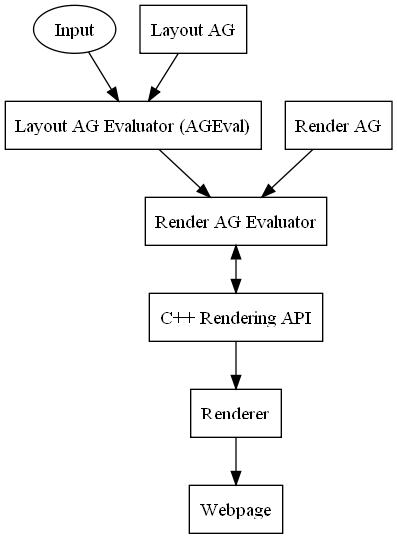
\includegraphics[width=200px]{BrowserFlow.png} }
\end{center}

It is assumed that there is some oracle that produces an evaluation/visit sequence that fully evaluates $t$ and computes the layout, this will be referred to as AGEval. When a new $l_i$ is available, the dynamic field's value is set to $l_i$. There is likewise an oracle that produces the visit sequence to traverse a given rendering AG input.

HTML will be scaled down to stackable, colored boxes with margins simulated by clear boxes. The boxes will also have a predefined width that applies to all boxes. Thus, all layout evaluation will pertain to calculation of y coordinates and height values. This limited version shall be referred to as HTML0 henceforth.

The proof will consider three attribute grammars. One representing attribute layout of HTML0 and two attribute grammars representing rendering. One for simple rendering and one to support incremental rendering.

\subsection{Layout Grammar}

The layout grammar will evaluate all attributes to completion, the same grammar will be used for both simple and incremental execution flows. The Root class represents the browser window, while the other implementations of Node represents physical boxes on the page. The VNode class allows for vertical stacking of child Nodes. Since every box has a fixed, inherited width, it does not make sense to have a HNode for horizontal stacking. A list of many children Nodes can be represented using nested VNodes. VNodeD is a duplicate of VNode that will become useful for incremental rendering. A LeafNode is a leaf in the semantic tree, it has no children and a defined height. Margins are represented by the EmptyNode class.
 
\begin{quote}
\begin{lstlisting}
Interface Frame{
	attrib pageHeight;
}

Interface Node{
	attrib x, y, w, h;
	field color;
}

Class Root implements Frame{
	field x, y, w, prefh, color;
	attrib uniqueID;
	uniqueID = getID();
	Node child;
	child@x = x;
	child@y = y;
	child@w = w;
	pageHeight = max(prefh, child@h);
}

Class VNode implements Node{
	attrib temph, uniqueID;
	Node child1;
	Node child2;
	uniqueID = getID();
	child1@x = x;
	child2@x = x;
	child1@w = w;
	child2@w = w;
	child1@y = y;
	temph = child1@h;
	child2@y = y + temph;
	h = temph + child2@y;
}

Class VNodeD implements Node{
	attrib temph, uniqueID;
	Node child1;
	Node child2;
	uniqueID = getID();
	child1@x = x;
	child2@x = x;
	child1@w = w;
	child2@w = w;
	child1@y = y;
	temph = child1@h;
	child2@y = y + temph;
	h = temph + child2@y;
}

Class LeafNode implements Node{
	attrib uniqueID;
	uniqueID = getID();
	field th;
	h = th;
}

Class EmptyNode implements Node{
	field th = 0, color = clear;
	h = th;
}
\end{lstlisting}
\end{quote}

The output of AGEval when given the sample input with $t[0]$ is as follows:

\begin{quote}
\begin{lstlisting}
Root{x: 0,
	 y: 0,
	 w: 480,
	 prefh: 400,
	 h: 400,
	 color: blue,
	 uniqueID: 0,
	 child: VNode{x: 0,
				  y: 0, 
				  w: 480,
				  h: 250,
				  color: green,
				  temph: 100,
				  uniqueID: 1,
				  child1: VNode{x: 0,
								y: 0, 
								w: 480,
								h: 100,
							    color: red,
							    temph: 50,
								uniqueID: 2,
							    child1: EmptyNode{x: 0,
												  y: 0, 
												  w: 480,
												  h: 50,
												  th: 50,
												  color: clear
										},
								child2: LeafNode{x: 0,
												 y: 50, 
												 w: 480,
												 h: 50,
												 th: 50,
												 color: yellow,
												 uniqueID: 3
										}
						  },
				  child2: VNodeD{x: 0,
								 y: 100, 
								 w: 480,
								 h: 150,
                                 color: indigo,
                                 temph: 100,
								 uniqueID: 4,
							     child1: VNode{x: 0,
											   y: 100, 
											   w: 480,
											   h: 100,								   
											   color: orange,
											   temph: 50,
											   uniqueID: 5,
											   child1: EmptyNode{x: 0,
																 y: 100, 
																 w: 480,
																 h: 50,
																 th: 50,
																 color: clear
													   },
											   child2: LeafNode{ x: 0,
																 y: 150, 
																 w: 480,
																 h: 50,
																 th: 50,
															     color: purple,
															     uniqueID: 6
													  }
										},
								 child2: VNode{x: 0,
											   y: 200, 
											   w: 480,
											   h: 50,								   
											   color: black,
											   temph: 50,
											   uniqueID: 7,
											   child1: EmptyNode{x: 0,
																 y: 200, 
																 w: 480,
																 h: 50,
																 th: 50,
																 color: clear
												       },
											   child2: EmptyNode{x: 0,
																 y: 250, 
																 w: 480,
																 h: 0,
																 th: 0,
																 color: clear
													   }
										}
						  }
			}
}
\end{lstlisting}
\end{quote}

\subsection{Simple Rendering Grammar}

The rendering grammar will take the completely evaluated semantic tree, thus, all the completed attributes in the layout AG are now fields. It will then proceed to render every node individually to the screen. In the simple case, note that VNodeD is a duplicate of VNode.

\begin{quote}
\begin{lstlisting}
Interface Frame{
	field pageHeight;
}

Interface Node{
	attrib g, v;
	field x, y, w, h, color;
}

Class Root implements Frame{
	field x, y, w, prefh, color, child, uniqueID;
	g = renderRoot(x, y, uniqueID);
	renderImage(g, x, y, w, pageheight, color, uniqueID);
	child@g = g;
	v = child@v;
	finishRoot(g, v);
}

Class VNode implements Node{
	field temph, child1, child2, uniqueID;
	renderImage(g, x, y, w, h, color, uniqueID);
	child1@g = g;
	child2@g = g;
	v = child1@v + child2@v;
}

Class VNodeD implements Node{
	field temph, child1, child2, uniqueID;
	renderImage(g, x, y, w, h, color, uniqueID);
	child1@g = g;
	child2@g = g;
	v = child1@v + child2@v;
}

Class LeafNode implements Node{
	field th, h, uniqueID;
	v = renderImage(g, x, y, w, h, color, uniqueID);
}

Class EmptyNode implements Node{
	field th, color;
	v = y; // nothing to render
}
\end{lstlisting}
\end{quote}

Given the sample input, $t[0]$ would produce the following rendering trace (after going through the API):
\begin{quote}
\begin{lstlisting}
group* g = createGroup();
g->x = 0;
g->y = 0;
g->zIndex = 0;
g[0] = g;
disableGroupDL(g);
myImgs[0] = addImage1(g, -1, 0, 0, 0, 480, 400, 0.0, 0.0, 1.0, 1.0);
myImgs[1] = addImage1(g, -1, 0, 0, 1, 480, 250, 0.0, 1.0, 0.0, 1.0);
myImgs[2] = addImage1(g, -1, 0, 0, 2, 480, 100, 1.0, 0.0, 0.0, 1.0);
myImgs[3] = addImage1(g, -1, 0, 50, 3, 480, 50, 1.0, 1.0, 0.0, 1.0);
myImgs[4] = addImage1(g, -1, 0, 100, 4, 480, 150, 1.0, 0.647f, 0, 1.0);
myImgs[5] = addImage1(g, -1, 0, 100, 5, 480, 100, 0.0, 0.808f, 0.820f, 1.0);
myImgs[6] = addImage1(g, -1, 0, 150, 6, 480, 50, 0.416f, 0.353f,0.808f, 1.0);
myImgs[7] = addImage1(g, -1, 0, 200, 7, 480, 50, 0.0, 0.0, 0.0, 1.0);
recalculateGroupBounds(g);
drawPage();
\end{lstlisting}
\end{quote}

$t[1]$ would produce:

\begin{quote}
\begin{lstlisting}
group* g = g[0];
g->x = 0;
g->y = 0;
g->zIndex = 0;
myImgs[0] = setTo(g, -1, 0, 0, 0, 480, 400, 0.0, 0.0, 1.0, 1.0);
myImgs[1] = setTo(g, -1, 0, 0, 1, 480, 249, 0.0, 1.0, 0.0, 1.0);
myImgs[2] = setTo(g, -1, 0, 0, 2, 480, 99, 1.0, 0.0, 0.0, 1.0);
myImgs[3] = setTo(g, -1, 0, 49, 3, 480, 50, 1.0, 1.0, 0.0, 1.0);
myImgs[4] = setTo(g, -1, 0, 99, 4, 480, 150, 1.0, 0.647f, 0, 1.0);
myImgs[5] = setTo(g, -1, 0, 99, 5, 480, 100, 0.0, 0.808f, 0.820f, 1.0);
myImgs[6] = setTo(g, -1, 0, 149, 6, 480, 50, 0.416f, 0.353f,0.808f, 1.0);
myImgs[7] = setTo(g, -1, 0, 199, 7, 480, 50, 0.0, 0.0, 0.0, 1.0);
recalculateGroupBounds(g);
drawPage();
\end{lstlisting}
\end{quote}

\subsection{Display Lists}
A display list is a sequence of commands compiled together for a graphics card to execute. This is used extensively in the field of graphics as the speedup is very significant given a large enough input. We are interested in applying this concept for browser rendering. Our initial benchmarks show that rendering the Slashdot front page with display lists naively (grouping every 20 or so boxes into a display list) was approximately 2x faster than doing so without display lists. We believe that more strategic usage of display lists will yield even more impressive results. The figure below illustrates the potential benefit of using display list rendering. Objects that are in a display list are always rendered exactly the same, relative to the display list. Essentially, instead of redrawing components individually, packaging components into the display list allows the GPU to "move" all the components at once (since the instructions are already compiled). 

\paragraph {Without Display Lists:}
\begin{center} \setlength\fboxsep{0pt}
\setlength\fboxrule{0.5pt}
\fbox{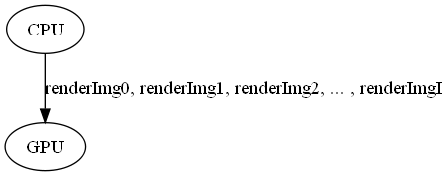
\includegraphics[width=200px]{NoDisplayList.png} }
\end{center}

\paragraph {With Display Lists:}
\begin{center} \setlength\fboxsep{0pt}
\setlength\fboxrule{0.5pt}
\fbox{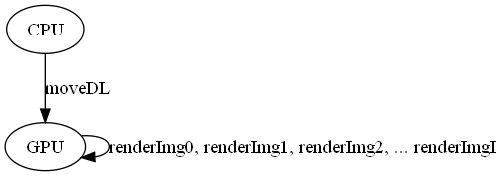
\includegraphics[width=200px]{DisplayList.png} }
\end{center}

\subsection{Incremental Rendering Grammar}

The incremental version of the rendering AG takes advantage of the display lists to improve rendering performance. The grammar is identical to the simple rendering AG except for the VNodeD class. The VNodeD class behaves differently based on whether it is the first frame or not. If it is the first frame, it must add the entire subtree of the VNodeD class into a display list. However, on subsequent frames, the entire subtree past the root can be ignored since the entire display list is moved.

Thus for the first frame:
\begin{quote}
\begin{lstlisting}
Class VNodeD implements Node{
	field temph, child1, child2, uniqueID;
	attrib g2, vtemp;
	g2 = renderDL(x, y, uniqueID);
	renderImage(g2, x, y, w, h, color, uniqueID);
	child1@g = g2;
	child2@g = g2;
	vtemp = child1@v + child2@v;
	v = finishDL(g2, vtemp);
}
\end{lstlisting}
\end{quote}

And for the further frames:
\begin{quote}
\begin{lstlisting}
Class VNodeD implements Node{
	field temph, child1, child2, uniqueID;
	attrib g2;
	g2 = moveDL(x, y, uniqueID);
	v = getNumber(g2);
\end{lstlisting}
\end{quote}

Given the sample input, $t[0]$ would produce the following rendering trace:
\begin{quote}
\begin{lstlisting}
group* g = createGroup();
g->x = 0;
g->y = 0;
g->zIndex = 0;
g[0] = g;
disableGroupDL(g);
myImgs[0] = addImage1(g, -1, 0, 0, 0, 480, 400, 0.0, 0.0, 1.0, 1.0);
myImgs[1] = addImage1(g, -1, 0, 0, 1, 480, 250, 0.0, 1.0, 0.0, 1.0);
myImgs[2] = addImage1(g, -1, 0, 0, 2, 480, 100, 1.0, 0.0, 0.0, 1.0);
myImgs[3] = addImage1(g, -1, 0, 50, 3, 480, 50, 1.0, 1.0, 0.0, 1.0);
group* g2 = createGroup();
g2->x = 0;
g2->y = 100;
g2->zIndex = 4;
g[4] = g2;
myImgs[4] = addImage1(g2, -1, 0, 0, 0, 480, 150, 1.0, 0.647f, 0, 1.0);
myImgs[5] = addImage1(g2, -1, 0, 0, 1, 480, 100, 0.0, 0.808f, 0.820f, 1.0);
myImgs[6] = addImage1(g2, -1, 0, 50, 2, 480, 50, 0.416f, 0.353f,0.808f, 1.0);
myImgs[7] = addImage1(g2, -1, 0, 100, 3, 480, 50, 0.0, 0.0, 0.0, 1.0);
recalculateGroupBounds(g2);
recalculateGroupBounds(g);
drawPage();
\end{lstlisting}
\end{quote}

$t[1]$ would produce:

\begin{quote}
\begin{lstlisting}
group* g = g[0];
g->x = 0;
g->y = 0;
g->zIndex = 0;
myImgs[0] = setTo(g, -1, 0, 0, 0, 480, 400, 0.0, 0.0, 1.0, 1.0);
myImgs[1] = setTo(g, -1, 0, 0, 1, 480, 249, 0.0, 1.0, 0.0, 1.0);
myImgs[2] = setTo(g, -1, 0, 0, 2, 480, 99, 1.0, 0.0, 0.0, 1.0);
myImgs[3] = setTo(g, -1, 0, 49, 3, 480, 50, 1.0, 1.0, 0.0, 1.0);
group* g2 = g[4];
g2->x = 0;
g2->y = 99;
recalculateGroupBounds(g2);
recalculateGroupBounds(g);
drawPage();
\end{lstlisting}
\end{quote}

\section{Proof of Consistency}
We must prove that given a valid input $t[l_0], t[l_1], ... t[l_n]$ the rendering trace of the incremental evaluation\\$E_{IR}(E_L(t[l_0])).E_{IR}(E_L(t[l_1])). ... .E_{IR}(E_L(t[l_n]))$ is consistent with that of the simple evaluation\\ $E_{SR}(E_L(t[l_0])).E_{SR}(E_L(t[l_1])). ... .E_{SR}(E_L(t[l_n]))$. Consistency is defined as having identical screen representations over the duration of the input. Consistency will be maintained if the rendering trace of the incremental evaluation path can be reduced to the rendering trace resulting from the simple evaluation path.

\subsection{Input}

Our input $inp$ consists of a semantic tree $t$ and a list of values $l$.
\begin{definition}
Let $inp = \{t, [l_0, l_1, ..., l_{size}]\}$.
\end{definition} 

First, all attributes in $t$ must be evaluated by the end of the layout grammar.

\begin{definition}
A semantic tree $t$ is \underline {fully attributable} if $\forall a \in t'.$attributes$ | t'=$ AGEval$(t).$ (isEvaluated($a$) = true).
\end{definition}

At any point in time, the grammars will be analyzing an input for a specific frame, which is a semantic tree where the dynamic attribute has been replaced with a value.

\begin{definition}
Let $t[l_i] = t[dynamic=l_i]$.
\end{definition}

Since we are assuming a dynamic input, no $t$ is actually fully attributable, since fields labeled dynamic have no value. Thus, an input $inp$ is fully attributable if each $t[l_i]$ yields a fully attributable tree.

\begin{definition}
An input $inp$ is fully attributable if $\forall i \in l.$size. $t[l_i]$ is fully attributable.
\end{definition}

For the proof, we will consider only fully attributable dynamic inputs. Thus we assume that the input will contain a VNodeD that gives the renderer the root of the display list.

\begin{definition}
Let $I$ denote the set of all $inp$ s.t. $inp$ is fully attributable and contains a VNodeD.
\end{definition}

\subsection{Grammar Execution}

Now we define the execution of the grammars. There are two total execution flows, one simple and one incremental. Note that both flows go through the same layout AG evaluator (previously denoted AGEval) $E_L$. There are two evaluators for rendering: one for the simple rendering AG $E_{SR}$, and one for the incremental renderering AG $E_{IR}$. Since both evaluation paths use the same layout evaluator, we can abstract it out.

\begin{definition}
Let $t'[l_i] = E_L(t[l_i])$.
\end{definition}

Finally we define execution of the grammars over the entire input, which is simply a concatenation (".") over all the executions per frame.
\begin{definition}
Let Simple($inp$) = $E_{SR}(t'[l_0]).E_{SR}(t'[l_1]).$ $...$ $.E_{SR}(t'[l_i])$).
\end{definition}
\begin{definition}
Let Increm($inp$) = $E_{IR}(t'[l_0]).E_{IR}(t'[l_1]).$ $...$ $.E_{IR}(t'[l_i])$).
\end{definition}

\subsection{Reductions}
The definition of display lists allows us to assume the following reductions:

\begin{enumerate}
\item Adding an image in a display list reduces to adding an image outside a display list.
\begin{quote} renderImage$(g_i, x, y, ...)$ reduces to renderImage$(g_0, x, y,...)$ where $g_0$ is disabled.\end{quote}
\item Moving a display list $D$ from $[x, y]$ to $[x', y']$ reduces to redrawing each element in the display list.
\begin{quote} $\forall n[x=x_n, y=y_n] \in D.contents$. $n.x=x_n + (x'-x); n.y=y_n + (y'-y)$. \end{quote}
\end{enumerate}

\subsection{Theorems}

\begin{lemma} Given $t'[l_i], E_{SR}$ and $E_{IR}$ create identical rendering instructions until a VNodeD class is encountered. \end{lemma}
\begin{proof}
This case can be trivially done by case. For all classes other than VNodeD, the rendering instructions produced are identical. Thus as long as a VNodeD class has not been entered, it can be shown that the rendering instructions will be identical.
\end{proof}

\begin{lemma} Given $t'[l_i], E_{SR}$ and $E_{IR}$ create identical rendering instructions after a VNodeD subtree is finished evaluating. \end{lemma}
\begin{proof}
This requires showing that the calls in the VNodeD class do not have any side effects that impact any node outside of the VNodeD subtree. The only differing side effect of a VNodeD class is the creation of a group* that represents a display list. However, it can be seen in all classes that display lists $(g)$ are only passed in a inherited pattern, i.e. a parent never looks at its child's display lists. Therefore, it is impossible for any node outside VNodeD to access the display list unless it had the correct uniqueID, which is unique and only privately accessible to the root VNodeD class. Thus because all rendering instructions outside a VNodeD class are identical and the side effects during VNodeD's execution do not affect instructions in nodes outside the VNodeD subtree, the rendering instructions will be are identical for all classes outside a VnodeD subtree.
\end{proof}

% No longer needed as the reduction covers this
% \begin{lemma} Given an $inp'_0$ within a VNodeD subtree, renderImage$_{increm}$($g2..$) reduces to \\ renderImage$_{simple}(g..$). \end{lemma}
% \begin{proof}
% First a summary of what we know:
% \begin{itemize}
% \item Since we are within a VNodeD subtree, we know that the group g2 is enabled.
% \item No groups are enabled in simple rendering, so we know that g is disabled.
% \item The current class has fields $[x', y', w', h', color', uniqueID']$. Since these are a result of executing AGEval, these are the same for both rendering executions. 
% \item AddImage(g, x, y...) expects x, y coordinates relative to the position of g.
% \end{itemize}
% A valid reduction would be to replace $g2$ with $g$. To show this is valid, we must show that the final drawing coordinates are identical.
% In the simple case with $g$, the last case of renderImage will be executed, resulting in an image drawn at $(x', y')$.
% In the incremental case with $g2$, the first case of renderImage will be executed, resulting in coordinates $(g2->x + (x' - g2->x), g2->y + (y' - g2->y)) = (x', y')$.
% Note that any coordinate for $g2$ are irrelevant by AddImage as a result of renderImage. Replacing $g2$ with $g'$ will result in the same execution as the simple case, and the image will be drawn at $(x', y')$. Therefore, we have shown a reduction from the incremental to simple rendering function call to renderImage.
% \end{proof}

\begin{theorem} Given $t'[l_0], E_{IR}(t'[l_0])$ reduces to $E_{SR}(t'[l_0])$. \end{theorem}
\begin{proof}
By Lemma 4.1 and 4.2, we know that the rendering trace will be identical outside of a VNodeD subtree. Thus we must only prove that the trace created by the VNodeD class subtree in $E_{IR}$ reduces to the corresponding trace created by $E_{SR}$.
First we consider the trace for the VNodeD class. Rendering the VNodeD node in the display list reduces to doing so outside the display list by Reduction 1.\\
For the subtree, we just need to invoke Reduction 1 on all calls to renderImage() from nodes in the subtree.
Since all of the trace from $E_{IR}$ is either identical or reducable to the $E_{SR}$ trace for $t[l_0]$, it must be that the entire rendering trace for $E_{IR}(t'[l_0])$ reduces to $E_{SR}(t'[l_0]))$. 
\end{proof}

\begin{theorem} Given $t'[l_0]...t['l_{i+1}], E_{IR}(t[l_{i+1}]$) reduces to $E_{SR}(t[l_{i+1}]$). \end{theorem}
\begin{proof}
As in the proof above, Lemma 4.1 and 4.2 are invoked for situations where evaluation is outside of a VNodeD subtree. As for the subtree, we must show that the moveDL() command can be reduced to redrawing all the images in the subtree. Since $t'[l_0]$ gives us initial x, y coordinates for the display list and subtree elements, Reduction 2 can be invoked repeatedly to derive where to draw all subtree elements for the $(i+1)^{th}$ frame. 
\end{proof}

\begin{theorem} $\forall inp \in I. $Increm$(inp)$ is consistent with to Simple$(inp)$. \end{theorem}
\begin{proof}
Choosing an arbitrary $inp$, we must show that [$E_{IR}(t'[l_0]).E_{IR}(t'[l_1]).$ $...$ $.E_{IR}(t'[l_{size}])$] reduces to [$E_{SR}(t'[l_0]).E_{SR}(t'[l_1]).$ $...$ $.E_{SR}(t'[l_.{size}])$].\\
This will be done by strong mathematical induction on the frame number.\\
\emph{Base case:} Prove that $E_{IR}(t'[l_0])$ reduces to $E_{SR}(t'[l_0])$.\\
This was proven above in Theorem 4.3.\\
\emph{Induction hypothesis:} Assume that $E_{IR}(t'[l_0]$). $...$ . $E_{SR}(t'[l_i]$) reduces to $E_{SR}(t'[l_0])$. $...$ . $E_{SR}(t'[l_i])$).
\emph{Induction step:} We must prove that $E_{IR}(t'[l_{i + 1}])$ reduces to $E_{SR}(t[l_{i + 1}])$.\\
This is proven in Theorem 4.4.\\
Thus we have shown that for a valid input, the incremental execution reduces to the simple execution.
\end{proof}

Since the rendering instructions of the incremental flow reduce to those of the simple flow, it must be that the rendering output for all frames is identical.

\section{Conclusion}
We have demonstrated the reduction from the evaluation of the incrementalized grammar to that of the simple grammar, showing that display lists are a more efficient alternative to rendering individual images. Future work will be in many forms. First, we must explore algorithms to automatically determine where display lists should be created. Second, incrementalization must be integrated with our existing attribute grammar evaluation system. Third, we must extend the simple HTML0 to encompass both height and width, which will introduce another dimension of complexity. Finally, we must support arbitrary numbers of dynamic properties, meaning that the input will be a sequence of entire semantic trees.

This paper describes one of two core aspects in our approach to browser page layout, the other aspect being layout evaluation specialization (abstracted away as AGEval in this paper). It is hoped that a combination of these two techniques will allow for more efficient page layout and rendering, allowing for greater accessibility and power savings on mobile platforms.

\section{Appendix}

\subsection{Supporting C++ File}

The following file contains all supporting functions for utilized by the layout and rendering attribute grammars. Note that the file is also responsible for remembering state between frames, currently achieved through global variables.

\begin{quote}
\begin{lstlisting}
int counter = 0;
int id = 0;
HashMap<int, group*> groups;
HashMap<int, img1*> images;

int max(int v1, int v2){
	return max(v1, v2);
}

int getID(){
	int val = id;
	id++;
	return val;
}

group* renderRoot(int x, int y, int ID){
	group* g;
	if (!groups.hasKey(ID)){
		g = createGroup();
		disableGroupDL(g);
		groups.put(ID, g);
	}
	else {
		g = groups.get(ID);
	}
	g->x = r->x;
	g->y = r->y;
	g->zIndex = 0;
	return g;
}

group* renderDL(int x, int y, int ID){
	group* g;
	if (!groups.hasKey(ID)){
		g = createGroup(); // do not disable
		groups.put(ID, g);
	}
	else{
		g = groups.get(ID);
	}
	g->x = x;
	g->y = y;
	g->zIndex = ID;
	return g;
}

void finishRoot(group* g, int v){
	recalculateGroupBounds(g);
	drawPage();
}

int finishDL(group* g, int v){
	recalculateGroupBounds(g);
	return g->y;
}

int getNumber(group* g){
	return g->x;
}

int renderImage(group* g, int x, int y, int w, int h, Color color, int ID){
	if (g.isEnabled()){
		// guaranteed !images.hasKey(ID) since will only call this on 1st pass
		img1* img = 
			addImage1(g, -1, (x - g->x), (y - g->y), 
				(counter - g->zIndex), w, h, 0, 0, 0, 0);
		img->changeColor(color);
		images.put(ID, img);
		return counter++;
	}
	if (images.hasKey(ID)){
		img1* myImg = images.get(ID);
		myImg->x = x;
		myImg->y = y;
		myImg->h = h;
		myImg->w = w;
		myImg->changeColor(color);
	}
	else {
		img1* img = addImage1(g, -1, x, y, counter, 
						w, h, 0, 0, 0, 0);
		img->changeColor(color);
		images.put(ID, img);
		return counter ++;
	}
}

// only legal if DL with ID exists
group* moveDL(int x, int y, int ID){
	group* g = groups.get(ID);
	g->x = x;
	g->y = y;
}
\end{lstlisting}
\end{quote}

\bibliography{biblio}
\bibliographystyle{plain}
\end{document}